\pagestyle{plain} % No headers, just page numbers

% Local macros (matching the AISTATS 2025 paper notation)
\newtheorem{proposition}{Proposition}[chapter]
\newtheorem{lemma}{Lemma}[chapter]
\theoremstyle{definition}
\newtheorem{fact}{Fact}[chapter]
\theoremstyle{plain}
\newcommand{\uni}{\mathcal{U}}
\newcommand{\epsi}{\epsilon}
\newcommand{\opt}{\textsc{OPT}}
\newcommand{\marge}[2]{\Delta \left( #1 \mid #2 \right)}
\newcommand{\nhi}{\textsc{NHI}}
\newcommand{\qss}{\textsc{QuickPrune-Single}}

\chapter{\uppercase {QuickPrune: Theoretically Grounded Pruning of Large Ground Sets}} \label{chap:quickprune}

Prior to our work, all existing pruning methods were heuristics with no formal performance
guarantees. It was unknown whether it was even possible to efficiently produce a pruned
ground set with provable bounds on both its size and the fraction of optimal value it
retains. In this chapter, we introduce QuickPrune~\citep{pmlr-v258-nath25a}, a lightweight
pruning algorithm for constrained discrete optimization that processes elements in a
single pass through the ground set, discarding those unlikely to appear in an optimal
solution. Under mild assumptions on the objective function and element costs, we prove
that the pruned ground set retains a constant fraction of the optimal value across a
range of budgets, while its size grows only logarithmically in the original ground set.
QuickPrune is the first pruning algorithm to provide such guarantees, and the first to
support a range of budgets simultaneously rather than a single budget instance.

\begin{figure}[t]
  \centering
  \begin{subfigure}[b]{0.48\textwidth}
    \centering
    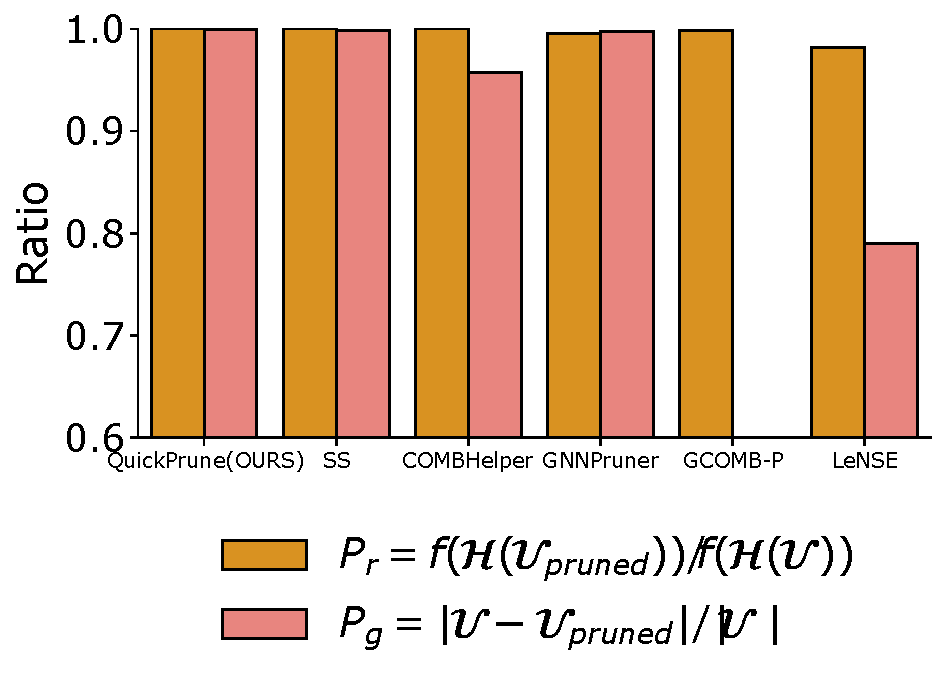
\includegraphics[width=\textwidth]{figures/quickprune/MaxCover_performance.pdf}
    \caption{Typical empirical results of QuickPrune versus competing methods on an
      instance of the Maximum Cover problem: QuickPrune retains 99.99\% of the optimal
      value while pruning 99.95\% of the ground set.}
    \label{fig:qp-maxcover}
  \end{subfigure}
  \hfill
  \begin{subfigure}[b]{0.48\textwidth}
    \centering
    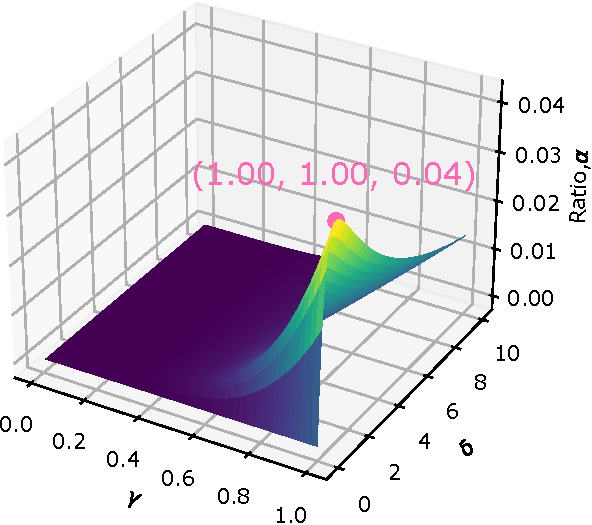
\includegraphics[width=\textwidth]{figures/quickprune/alpha_plot.pdf}
    \caption{Plot of the pruning ratio $\alpha(\epsilon, \delta, \gamma)$ of Theorem~2 as
      a function of the parameter $\delta$ and the $\gamma$-submodularity of the objective
      function $f$, with $\epsilon$ fixed to $0.01$.}
    \label{fig:qp-alpha}
  \end{subfigure}
  \caption{Overview of QuickPrune performance and theoretical guarantees.}
  \label{fig:qp-intro}
\end{figure}

\section{Problem Setting}

QuickPrune operates under a general knapsack constraint: each element $e \in \mathcal{U}$
has a modular cost $c(e) > 0$, and a feasible solution $S$ must satisfy $c(S) \leq \kappa$
for a given budget $\kappa$. We denote the optimal value under budget $\kappa$ by
\[
f_{\kappa}(\mathcal{U}) = \max_{S \subseteq \mathcal{U} : c(S) \leq \kappa} f(S).
\]
Size constraints are a special case where $c(e) = 1$ for all $e$. A key requirement is
that pruning should be effective across a range of budgets
$[\kappa_{\min}, \kappa_{\max}]$, not just a single value, since the pruned set
permanently discards elements and should remain useful for downstream solvers under
varying budget scenarios.

\section{Key Assumptions}

Our theoretical guarantees rely on two assumptions on the objective function and the
problem instance.

\textbf{Monotone $\gamma$-Weak Submodularity.} The objective function $f$ is monotone
($\Delta(x \mid S) \geq 0$ for all $S \subseteq \mathcal{U}$, $x \notin S$) and
$\gamma$-weakly submodular, where $\gamma \in (0, 1]$ is the maximum value such that for
all $S \subseteq T \subseteq \mathcal{U}$ and all $x \notin T$,
\[
\gamma \cdot \Delta(x \mid T) \leq \Delta(x \mid S),
\]
where $\Delta(x \mid S) = f(S \cup \{x\}) - f(S)$ denotes the marginal gain of element
$x$ to set $S$. When $\gamma = 1$, $f$ is fully submodular. This is also known as the
diminishing-returns ratio. Submodularity is a notion of diminishing returns that is
satisfied or partially satisfied by many varied objective functions, and occupies a role
for discrete optimization analogous to the role of convexity in continuous optimization.

\textbf{No Huge Items (NHI) Assumption.} Given an instance $(f, c, \kappa)$ with
parameter $\eta > 0$, there exists an optimal solution $O$ such that for all $o \in O$,
$c(o) \leq \kappa(1 - \eta)$. Intuitively, this says that no single element of an
optimal solution consumes a very large fraction of the total budget. For the common case
of size constraints, this assumption is satisfied when $\kappa \geq 2$ and
$\eta \leq 1/2$.

\section{Algorithm}

QuickPrune operates at two levels. The single-budget algorithm (QuickPrune-Single)
handles one knapsack constraint, and the main algorithm (QuickPrune) runs multiple copies
in parallel to cover a range of budgets. We emphasize that lightweight pruning methods
are needed since an expensive pruning process defeats the purpose of pruning.

\subsection{QuickPrune-Single}

Given a single budget value $\kappa$ with parameters $\delta > 0$ (size-control) and
$\epsilon > 0$ (deletion), the algorithm takes one pass through $\mathcal{U}$ and
processes elements one-by-one. Once an element is rejected, it is never re-considered and
may be safely discarded. The full pseudocode is given in Algorithm~\ref{alg:single}.

\begin{algorithm}[t]
\caption{QuickPrune-Single: Pruning for a single constraint.}
\label{alg:single}
\begin{algorithmic}[1]
\REQUIRE Instance $(f, \mathcal{U}, c, \kappa)$, size-control parameter $\delta > 0$,
  deletion parameter $\epsilon > 0$
\ENSURE Pruned ground set $\mathcal{U}'$
\STATE $A \gets \emptyset$, $a^* \gets \emptyset$, $A_s \gets \emptyset$
\FOR{$e \in \mathcal{U}$}
  \IF{$c(e) > \kappa$}
    \STATE \textbf{continue}
  \ENDIF
  \IF{$\Delta(e \mid A) > \frac{\delta \, c(e) \, f(A)}{\kappa}$ \label{line:add}}
    \STATE $A \gets A \cup \{e\}$
  \ENDIF
  \IF{$f(e) > f(a^*)$}
    \STATE $a^* \gets e$
  \ENDIF
  \IF{$f(A) > \frac{n}{\epsilon} \cdot f(A_s)$ \label{line:delete}}
    \STATE $A \gets A \setminus A_s$ \label{line:delete-set}
    \STATE $A_s \gets A$
  \ENDIF
\ENDFOR
\RETURN $\mathcal{U}' \gets A \cup \{a^*\}$
\end{algorithmic}
\end{algorithm}

An element $e$ is added to the running set $A$ if its marginal gain satisfies
$\Delta(e \mid A) > \frac{\delta \, c(e) \, f(A)}{\kappa}$; intuitively, the element
must increase the value of $A$ by an amount proportional to its cost-to-budget ratio to be
worth retaining. When $A = \emptyset$ and $f(\emptyset) = 0$, the threshold is zero and
every element passes the condition, so the first element encountered is always added. The deletion step (Line 12) is the key mechanism for controlling the size
of $\mathcal{U}'$: when the accumulated value grows by a factor of $n / \epsilon$ since
the last checkpoint $A_s$, old elements are discarded. Submodularity bounds the amount of
value lost from each deletion, and the condition on element addition bounds the maximal
number of elements required for the increased value.

\subsection{QuickPrune (Main Algorithm)}

To handle a range of budgets $[\kappa_{\min}, \kappa_{\max}]$, QuickPrune generates a set
of budget values and runs multiple copies of QuickPrune-Single in parallel, one for each
budget. The full pseudocode is given in Algorithm~\ref{alg:multi}.

\begin{algorithm}[t]
\caption{QuickPrune: The main pruning algorithm.}
\label{alg:multi}
\begin{algorithmic}[1]
\REQUIRE Instance $(f, \mathcal{U}, c, [\kappa_{\min}, \kappa_{\max}])$, parameters
  $\delta > 0$, $\epsilon > 0$, $0 < \eta \leq 1/2$
\ENSURE Pruned ground set $\mathcal{U}'$
\STATE $\mathcal{B} = \{\tau_i = \kappa_{\max}(1 - \eta)^i :
  i \in \mathbb{Z}, \; (1 - \eta)\kappa_{\min} \leq \tau_i \leq \kappa_{\max}\}$
\STATE Initialize a copy $\mathcal{QP}_\tau$ of QuickPrune-Single for each
  $\tau \in \mathcal{B}$, with parameters $\epsilon, \delta$
\FOR{$e \in \mathcal{U}$}
  \STATE Pass $e$ to $\mathcal{QP}_\tau$ for all $\tau \in \mathcal{B}$
\ENDFOR
\RETURN the union of all sets returned by all instances $\mathcal{QP}_\tau$
\end{algorithmic}
\end{algorithm}

Each element of $\mathcal{U}$ is passed to all copies, and the final output is the union
of all pruned sets. This requires
$\mathcal{O}(\log(\kappa_{\max} / \kappa_{\min}))$ copies and the same number of queries
to $f$ per element processed.

\section{Theoretical Results}

We present the main theoretical result of this work. The proof proceeds by: (i) bounding
the size of $\mathcal{U}'$ via the geometric increase in $f(A)$ (Proposition 1);
(ii) bounding the value lost from deletion throughout execution (Proposition 2);
(iii) showing that a feasible set $A' \subseteq \mathcal{U}'$ exists with a constant
fraction of the optimal value (Lemma 1 and Proposition 3); and (iv) relating the value of
$\mathcal{U}'$ to the true optimum (Proposition 4).

\textbf{Theorem 1 (Single Budget).}\label{thm:single} Let QuickPrune-Single be run on instance
$(\mathcal{U}, c, f, \kappa)$ with parameters $\epsilon, \delta > 0$, such that $f$ is
monotone $\gamma$-weakly submodular. Then the algorithm produces $\mathcal{U}'$ such that
\[
|\mathcal{U}'| < 2\left(1 + \frac{\kappa}{\delta \, c_{\min}}\right)
\log(n / \epsilon) + 3,
\]
and there exists $A' \subseteq \mathcal{U}'$ with $c(A') \leq \kappa$ and
\[
f(A') \geq \frac{\delta \gamma^4 (1 - \epsilon \gamma^{-1})}
{2(\delta \gamma^2 + 1)(1 + \gamma^{-1} \delta)} \cdot f_{\kappa}(\mathcal{U}).
\]

\textbf{Theorem 2 (Multi-Budget, Main Result).} Let $\kappa_{\min} < \kappa_{\max}$, let
$0 < \eta \leq 1/2$, and let $f$ be monotone $\gamma$-weakly submodular and $c$ be a modular function,
respectively. Suppose that for all $\kappa' \in [\kappa_{\min}, \kappa_{\max}]$, the
instance $(f, c, \kappa')$ satisfies the NHI assumption with $\eta$. Let $\mathcal{U}'$
be the output of QuickPrune. Then, for all
$\kappa' \in [\kappa_{\min}, \kappa_{\max}]$:
\begin{itemize}
  \item \textbf{Value retention:}
    $f_{\kappa'}(\mathcal{U}') \geq
    \frac{\delta \gamma^5 (1 - \epsilon \gamma^{-1})}
    {6(\delta \gamma^2 + 1)(1 + \gamma^{-1} \delta)} \cdot f_{\kappa'}(\mathcal{U}).$
  \item \textbf{Size bound:}
    $|\mathcal{U}'| = \mathcal{O}\!\left(
    \log\!\left(\frac{\kappa_{\max}}{\kappa_{\min}}\right)
    \left(1 + \frac{\kappa_{\max}}{\delta \, c_{\min}}\right)
    \log(n / \epsilon)\right),$
    where $c_{\min} = \min_{u \in \mathcal{U}} c(u)$ and $n = |\mathcal{U}|$.
\end{itemize}
When $\gamma = 1$ (fully submodular) and $\delta = 1$, the value retention simplifies to
$f_{\kappa'}(\mathcal{U}') \geq (1/24 - \epsilon) \cdot f_{\kappa'}(\mathcal{U})$.

The key properties of QuickPrune are: (i) single-pass processing where each element is
considered once and never reconsidered; (ii) query complexity of
$\mathcal{O}(\log(\kappa_{\max} / \kappa_{\min}))$ per element; and (iii) pruned set size
that is logarithmic in the original ground set size $n$.

\subsection{Supporting Propositions}

\begin{fact} \label{fact:1}
  Let $(y_i)_{i=1}^m$ be a sequence of positive real numbers, such that, for some $\beta > 0$, it holds that $y_i \ge (1 + \beta)y_{i-1}$, for all $i \in [m]$. Let $\gamma > 0$. Then, if $m \ge \frac{\beta + 1}{\beta}\log \gamma^{-1} $, it holds that $y_m \ge y_1 / \gamma$.
\end{fact}

\begin{proposition} \label{prop:uprime-size}
  The size of $\uni'$, as returned by Alg.~\ref{alg:single}, satisfies
  $$|\uni'| < 2 \left( 1 + \frac{\kappa }{\delta c_{min} } \right) \log ( n / \epsi ) + 3,$$
  where $c_{min} = \min_{a \in \uni } c(a).$
\end{proposition}

\begin{proposition} \label{prop:ahat-adot}
  Suppose $f$ is $\gamma$-weakly submodular.
  Let $A_i$ be the value of $A$ after the execution of iteration $i$ of the \textbf{for} loop,
  for $i = 1$ to $n$, and $A_0 = \emptyset$.
  Let $\hat A = \bigcup A_j, \dot A = A_n$. Then $f( \dot A ) \ge (1 - \gamma^{-1} \epsi )f( \hat A)$.
\end{proposition}

\begin{lemma} \label{lemma:value-inside-A}
  Let $f$ be $\gamma$-weakly submodular.
  Let $\delta, \kappa > 0$. Suppose $A_i = \{ a_1, \ldots a_i \}$ is a sequence of sets satisfying
  (1) $c(a_i) \le \kappa$, and (2) $\marge{ a_i }{ A_{i - 1} } \ge \gamma \frac{\delta c( a_i ) f( A_{i -1 } ) }{ \kappa }$,
  for each $i$ from $1$ to $m$. Let $f( a^* ) \ge \max_{i \in [m]} f(a_i)$, and $c(a^*) \le \kappa$.
  Then there exists $A^* \subseteq A_m + a^*$, such that $c( A^* ) \le \kappa$, and
  $f( A^* ) \ge \frac{ \delta \gamma^4}{2(\delta\gamma^2 + 1)} f(A_m)$.
\end{lemma}

\begin{proposition} \label{prop:aprime}
  Let $\uni' = \dot A + a^*$ have its value at termination of \qss.
  There exists $A' \subseteq \uni' = \dot A + a^*$, such that $f(A') \ge \frac{\delta \gamma^4}{2(\delta \gamma^2 + 1)} f(\dot A )$
  and $c(A') \le \kappa$.
\end{proposition}

\begin{proposition} \label{prop:opt-ahat}
  Suppose Alg.~\ref{alg:single} is run on instance $(\uni,c,f,\kappa )$ with
  parameters $\delta, \epsi > 0$.
  Let $\hat A = \bigcup_{j \in [n]} A_j$ be all elements added to $A$.
  Then $f( \hat A ) \ge \opt / (1 + \gamma^{-1}\delta )$, where $\opt = \max_{S \subseteq \uni: c(S) \le \kappa } f(S).$
\end{proposition}

\subsection{Proof of Theorem~1}

\begin{proof}[Proof of Prop.~\ref{prop:uprime-size}]
  Let $m^* = \left( 1 + \frac{\kappa }{\delta c_{min} } \right) \log ( n / \epsi ) + 1.$

  First, we show that at any time during the execution of Alg.~\ref{alg:single}, $|A| \le m^* + |A_s|$.
  Fix a value $B$ of $A_s$, and let $A_i, 1 \le i \le m$ assume all distinct values of $A$ while $A_s$
  has value $B$, in the order in which they were assigned. Thus, $A_1 = A_s$, $A_2 = A_s + e_1, \ldots, A_m = A_s + e_1 + \ldots + e_{m-1}$.
  Then, let $(y_i = f(A_i))_{i=1}^m$. By Line \ref{line:add}, $y_i \ge \left( 1 + \frac{\delta c_{min}}{\kappa } \right) y_{i-1}$, for each $i \in [m]$. Let $\beta = \frac{\delta c_{min}}{\kappa }$; then by Fact \ref{fact:1}, if $i \ge m^* - 1$, then $y_i \ge \frac{n}{\epsi} y_1$, and a deletion is triggered on Line \ref{line:delete}, which changes the value of $A_s$. Hence, we have $m \le m^*$, which shows $|A| \le |A_s| = m^*$.

  Observe that after a deletion, $|A_s| = m \le m^*$. Since $A_s$ has initial value $\emptyset$, it holds that $|A_s| \le m^*$ throughout the execution of the algorithm. Therefore, $|A| \le 2m^*$, and thus $|\uni'| \le 2m^* +1$.
\end{proof}

\begin{proof}[Proof of Prop.~\ref{prop:ahat-adot}]
  Let $( \dot B_i )_{i=1}^m$ be the sequence of sets deleted by the algorithm on
  Line \ref{line:delete-set}, in the order in which they were deleted.
  Let $j(i)$ be the iteration of the \textbf{for} loop on which $B_i$
  was deleted, and let $A_{j(i)}$ be the value of the set $A$ at the
  beginning of iteration $j(i)$. Let $B_0 = \hat A$, and let
  $B_i = B_{i-1} \setminus \hat B_i$, for $i = 1$ to $m$.
  Observe that $B_m = \dot A$.

  We have that
  \begin{align*}
    f( B_{i-1} ) - f(B_i) &\overset{(a)}{\le} \gamma^{-1} f( \dot B_i ) \\
                          &\overset{(b)}{<} \frac{\gamma^{-1}\epsi}{n} f( A_{j(i)} ) \\
                          &\overset{(c)}{\le} \frac{\gamma^{-1}\epsi}{n} f( \hat A ),
  \end{align*}
  where Inequality (a) follows from $\gamma$-submodularity,
  Inequality (b) is from the condition to delete set $\dot B_i$ on Line \ref{line:delete},
  and Inequality (c) follows from monotonicity.
  From here,
  \begin{align*}
    f( \hat A ) - f( \dot A ) &= \sum_{i=1}^m f( B_{i-1} ) - f( B_i ) \\
    &\le m \cdot \frac{\gamma^{-1}\epsi}{n} f( \hat A ) \le \gamma^{-1}\epsi f( \hat A ). \qedhere
  \end{align*}
\end{proof}

\begin{proof}[Proof of Lemma \ref{lemma:value-inside-A}]
  If $c(A_m) \le \kappa$, let $A^* = A_m$ and there is nothing to show.
  Otherwise, let $A' =  \{a_{i'}, \ldots, a_m \}$, where $i' = \max_{i \in [m]} \{ i: c( \{ a_i, \ldots, a_m \} ) > \kappa \}$.
  We have
  \begin{align*}
    f(A') &\overset{(a)}{\ge} \gamma ( f(A_m) - f( A_m \setminus A') ) \\
          &\overset{(b)}{=} \gamma \sum_{i=i'}^m \marge{ a_i }{ A_{i-1} } \\
          &\overset{(c)}{\ge} \gamma^2 \sum_{i=i'}^m \frac{ \delta c(a_i) f( A_{i-1} )}{\kappa} \\
          &\overset{(d)}{>} \gamma^2 \delta f(A_{i'-1} ) = \gamma^2 \delta f( A \setminus A' ),
  \end{align*}
  where Inequality (a) follows from $\gamma$-submodularity and nonnegativity, Equality (b)
  is a telescoping sum, Inequality (c) is from the assumed condition (2), and Inequality
  (d) is from monotonicity and the fact that $c( A' ) > \kappa$.
  Thus
  \begin{align*}
    f(A_m) &\le \gamma^{-1} (f(A') + f( A_m \setminus A')) \\
           &< \gamma^{-1}(1 + 1/(\delta \gamma^2 )) f(A') = \frac{\delta \gamma^2  +1}{\delta \gamma^3 } f(A').
  \end{align*}
  Let $A'' = A' \setminus a_{i'}$; by choice of $A'$, it holds that $c(A'') \le \kappa$.
  Finally, from $\gamma$-submodularity,
  \begin{align*}
    f(a^*) + f(A'') &\ge f(a_{i'}) + f(A'') \\
                    &\ge \gamma f(A') \ge \frac{\delta \gamma^4}{\delta \gamma^2 + 1} f(A_m).
  \end{align*}
  Thus, set $A^* = \arg\max \{ f( a^* ), f(A'') \}$.
\end{proof}

\begin{proof}[Proof of Prop.~\ref{prop:aprime}]
  Let $\dot A = \{\dot a_1, \ldots, \dot a_m \}$ be in the order in which the elements were added into set $A$.
  That is, if $j(i)$ the iteration of the \textbf{for} loop in which $\dot a_i$ is considered, $i < i'$ implies
  $j(i) < j(i')$. Let $A_j$ be the value of the set $A$ at the beginning of iteration $j$ of the \textbf{for}
  loop.
  Then
  \begin{align*}
    \marge{ \dot a_i }{ \dot A_{i-1} } &\overset{(a)}{\ge} \gamma \marge{ \dot a_i }{ A_{j(i)} } \\
                                       &\overset{(b)}{\ge} \gamma \frac{ \delta c( \dot a_i ) f( A_{j(i)} )}{\kappa} \\
                                       &\overset{(c)}{\ge} \gamma \frac{ \delta c( \dot a_i ) f( \dot A_{i - 1} )}{\kappa},
  \end{align*}
  where (a) follows from $\gamma$-submodularity since $\dot A_{i-1} \subseteq A_{j(i)}$,
  (b) follows from the condition on Line \ref{line:add},
  (c) follows from monotonicity.
  Also $c(\dot a_i ) \le \kappa$, for all $i$. Therefore, $\dot A_i$ and $a^*$ satisfy the conditions of
  Lemma \ref{lemma:value-inside-A}, which implies the result.
\end{proof}

\begin{proof}[Proof of Prop.~\ref{prop:opt-ahat}]
  Let $O \subseteq \uni$, such that $c(O) \le \kappa$ and $f(O) = \opt$.
  For each $e \in \uni$, let $j(e)$ be the iteration of the \textbf{for}
  loop in which $e$ was considered, and let $A_j$ be the value of the set
  $A$ at the beginning of the $j$th iteration.
  Then
  \begin{align*}
    \opt - f( \hat A ) &\overset{(a)}{\le } f( O \cup \hat A ) - f( \hat A) \\
                       &\overset{(b)}{\le } \gamma^{-1} \sum_{o \in O \setminus \hat A} \marge{o}{ A_{j(o)} } \\
                       &\overset{(c)}{<} \gamma^{-1} \sum_{o \in O \setminus \hat A} \frac{\delta c(o) f(A_{j(o)})}{\kappa } \\
                       &\overset{(d)}{\le} \gamma^{-1} \sum_{o \in O \setminus \hat A} \frac{\delta c(o) f( \hat A )}{\kappa } \\
                       &\overset{(e)}{\le} \gamma^{-1} \delta f( \hat A ),
  \end{align*}
  where (a) follows from monotonicity,
  (b) follows from $\gamma$-submodularity,
  (c) holds since the condition on Line \ref{line:add} must have failed since $o \not \in \hat A$,
  (d) follows from monotonicity, and (e) holds since $\sum_{o \in O} c(o) \le \kappa$.
\end{proof}

\begin{proof}[Proof of Theorem \ref{thm:single}]
  Finally, we are ready to put all the pieces together.
  Assume the hypotheses of the theorem statement.
  The size bound on $\uni'$ follows by Proposition \ref{prop:uprime-size}.
  Let $A_j$ be the value of the set
  $A$ at the beginning of the $j$th iteration of \qss.
  Let $\dot A = A_{n+1}$ be the final value of $A$,
  $\hat A = \bigcup_{i \in [n + 1]} A_i$.
  Let $A'$ be as guaranteed by Proposition \ref{prop:aprime}.
  Then $f(A') \overset{(a)}{\ge} \frac{\delta \gamma^4 }{2(\delta \gamma^2 + 1)} f( \dot A )
  \overset{(b)}{\ge} \frac{\delta \gamma^4(1 - \epsi \gamma^{-1})}{2(\delta \gamma^2 + 1)} f( \hat A )$,
  where (a) is by Prop.~\ref{prop:aprime},
  (b) is by Prop.~\ref{prop:ahat-adot},
  and the result follows from Prop.~\ref{prop:opt-ahat}.
\end{proof}

\subsection{Proof of Theorem~2}

\begin{proposition} \label{prop:part}
  Suppose instance $(f,c,\kappa)$ satisfies the \nhi assumption
  with $0 < \eta \le 1/2$.
  Then, there exists an optimal solution $O$ to the instance, such
  that $O$ can be partitioned into at most three sets $\{ O_i : i \in [3] \}$, such
  that $c(O_i) \le \kappa (1 - \eta )$, for each $i \in [3]$.
\end{proposition}

\begin{proof}[Proof of Prop.~\ref{prop:part}]
  Let $X \subseteq O$ be a maximal subset with $c(X) \le \kappa ( 1 - \eta )$.
  By Assumption \nhi, $X \neq \emptyset$. If $X = O$, there is nothing to show.
  Otherwise, let $o \in O \setminus X$. By definition, $c \left( O \setminus (X \cup \{ o \} \right) < \kappa - \kappa ( 1 - \eta ) = \eta \kappa < (1 - \eta) \kappa$, since $\eta \le 1/2$. Therefore, $O_1 = X$, $O_2 = \{ o \}$, and $O_3 = O \setminus (X \cup \{ o \} )$
  form the requisite partition.
\end{proof}

\begin{proof}[Proof of Theorem~2]
  Assume the hypotheses of the theorem, and let
  $\kappa' \in [\kappa_{\min}, \kappa_{\max}]$. By the choice of
  the set $\mathcal B$, there
  exists a $\tau \in \mathcal B$, such that $\kappa'(1 - \eta) \le \tau \le \kappa'$.
  Let $O \subseteq \uni$ be an optimal solution to $f_{\kappa'}( \uni )$
  satisfying Assumption \nhi. By Proposition \ref{prop:part}, $O$ can be partitioned
  into at most three sets $\{ O_i \}$, such that $c( O_i ) \le \kappa ( 1 - \eta ) \le \tau$.

  Moreover, by Theorem \ref{thm:single}, there exists $X \subseteq \uni'$, such that
  1) $c(X) \le \tau$, and
  2) $f(X) \ge
  \alpha f( O_i )$,
  with $\alpha =  \frac{\delta \gamma^4(1 - \epsi \gamma^{-1})}{2(\delta \gamma^2 + 1)( 1 + \gamma^{-1} \delta ) }$.
  Therefore, $3f(X) \ge \alpha \sum_{i = 1}^3 f( O_i ) \ge \alpha \gamma f(O)$, where the last inequality follows from submodularity.
  Thus, $f(X) \ge \alpha \gamma f(O) / 3$.
  Finally, the size bound on $\uni'$
  follows from Prop.~\ref{prop:uprime-size} and the size of $\mathcal B$.
\end{proof}

\section{Experimental Evaluation}

We compare the empirical performance of QuickPrune to existing methods for the pruning
problem across three graph CO problems, for both size and knapsack constraints.

\subsection{Experimental Setup}

\textbf{Applications.} All problems are defined on an undirected graph $G = (V, E)$ where
each node $v \in V$ has cost $c(v)$. We evaluate on three graph CO problems:

\begin{itemize}
  \item \textbf{Maximum Coverage (MaxCover):} Find $S \subseteq V$ with
    $\sum_{v \in S} c(v) \leq k$ maximizing
    $f(S) = |\{v \mid v \in S \lor \exists (u,v) \in E,\, u \in S\}|$,
    the number of vertices covered by $S$ and its neighbors.

  \item \textbf{Maximum Cut (MaxCut):} Find $S \subseteq V$ with
    $\sum_{v \in S} c(v) \leq k$ maximizing
    $f(S) = |\{(u,v) \in E : v \in S,\, u \in V \setminus S\}|$,
    the number of edges crossing the cut.

  \item \textbf{Influence Maximization (IM):} Given edge probabilities $p(u,v)$ and a
    cascade model, find $S \subseteq V$ with $\sum_{v \in S} c(v) \leq k$ maximizing
    $f(S) = \mathbf{E}[\sigma(S)]$, the expected spread. We use the independent cascade
    model~\citep{kempe2003maximizing}.

\end{itemize}

\textbf{Datasets.} We evaluate on eight real-world graphs from the Stanford Large Network
Dataset Collection (SNAP)~\citep{leskovec2016snap}, following the experimental setup
of~\citep{ireland2022lense}. The graphs range from small networks
(Facebook, $\sim$4K vertices) to large-scale graphs (Skitter, $\sim$1.7M vertices).

\textbf{Baselines.} We compare against: Submodular Sparsification (SS)~\citep{zhou2017scaling},
GCOMB~\citep{manchanda2020gcomb}, LeNSE~\citep{ireland2022lense},
COMBHelper~\citep{tian2024combhelper}, and GNNPruner, an ablation baseline that is a
simplified version of COMBHelper using a GNN with random node features instead of
hand-crafted features. For knapsack constraints, since the prior ML
methods do not easily generalize, we compare to GNNPruner and a Top-$k$ approach that
selects elements with the highest degree-to-cost ratios.

\textbf{Evaluation Metrics.} We evaluate using three metrics where higher values indicate
better performance: (1) the pruning approximation ratio
$P_r = f(\mathcal{H}(\mathcal{U}')) / f(\mathcal{H}(\mathcal{U}))$, measuring the
fraction of solution quality retained; (2) the pruned fraction
$P_g = |\mathcal{U} \setminus \mathcal{U}'| / |\mathcal{U}|$, measuring the fraction of
the ground set removed; and (3) the combined metric $C = P_r \cdot P_g$, which balances
both objectives. Since an algorithm could trivially achieve the highest score in one metric
by disregarding the other (pruning nothing or pruning everything), the combined metric
provides a balanced evaluation. Because computing $\opt$ exactly is intractable for these objectives, $\mathcal{H}$ is a
heuristic solver (Greedy for MaxCover/MaxCut, IMM for Influence Maximization) used as a
proxy for $\opt$; $P_r$ is therefore a lower bound on the true retention ratio, and the
absolute gap to $\opt$ is unknown.


\subsection{Results on Size Constraints}

For the size constraint experiments with budget $k = 100$, we observe that all algorithms
achieve similar pruning approximation ratios. However, QuickPrune prunes the ground set far more aggressively than most algorithms, often by orders of magnitude. Table~\ref{tab:size_constraint}
summarizes the results across all applications and datasets.

\begin{table}[t]
\centering
\caption{Comparison of pruning methods under size constraints ($k = 100$) across
  MaxCover, MaxCut, and Influence Maximization on eight SNAP graphs. $P_r$: fraction of
  solver objective retained after pruning; $P_g$: fraction of ground set removed;
  $C = P_r \cdot P_g$: combined metric balancing quality and reduction. Best $C$ per
  instance in bold; ``--'' indicates the method exceeded the time limit.
  *Values as reported in~\citep{ireland2022lense}.}
\label{tab:size_constraint}
\resizebox{\textwidth}{!}{%
\begin{tabular}{@{}l ccc ccc ccc ccc ccc ccc@{}}
\toprule
& \multicolumn{3}{c}{QuickPrune} & \multicolumn{3}{c}{SS} & \multicolumn{3}{c}{GCOMB*}
& \multicolumn{3}{c}{COMBHelper} & \multicolumn{3}{c}{LeNSE*} & \multicolumn{3}{c}{GNNPruner} \\
\cmidrule(lr){2-4}\cmidrule(lr){5-7}\cmidrule(lr){8-10}\cmidrule(lr){11-13}\cmidrule(lr){14-16}\cmidrule(lr){17-19}
Graph & $P_r$ & $P_g$ & $C$ & $P_r$ & $P_g$ & $C$ & $P_r$ & $P_g$ & $C$
& $P_r$ & $P_g$ & $C$ & $P_r$ & $P_g$ & $C$ & $P_r$ & $P_g$ & $C$ \\
\midrule
\multicolumn{19}{c}{\textbf{Maximum Cover}} \\
\midrule
Facebook  & 1.00 & 0.995 & \textbf{0.995} & 0.988 & 0.903 & 0.892 & 0.927 & 0.070 & 0.065 & 1.000 & 0.384 & 0.384 & 0.966 & 0.070 & 0.068 & 1.000 & 0.770 & 0.770 \\
Wiki      & 1.00 & 0.942 & \textbf{0.942} & 0.956 & 0.935 & 0.893 & 0.990 & 0.030 & 0.030 & 1.000 & 0.453 & 0.453 & 1.094 & 0.340 & 0.372 & 1.000 & 0.920 & 0.920 \\
Deezer    & 0.961 & 0.980 & 0.941 & 0.987 & 0.986 & \textbf{0.973} & 0.994 & 0.130 & 0.129 & 1.000 & 0.728 & 0.728 & 0.979 & 0.750 & 0.734 & 1.000 & 0.915 & 0.915 \\
Slashdot  & 1.00 & 0.993 & \textbf{0.993} & 0.982 & 0.989 & 0.972 & 1.000 & 0.020 & 0.020 & 1.000 & 0.984 & 0.984 & 0.979 & 0.690 & 0.676 & 1.000 & 0.981 & 0.981 \\
Twitter   & 0.993 & 0.991 & \textbf{0.984} & 0.931 & 0.989 & 0.921 & 0.997 & 0.170 & 0.170 & 1.000 & 0.565 & 0.565 & 0.989 & 0.330 & 0.326 & 0.999 & 0.979 & 0.978 \\
DBLP      & 0.995 & 0.996 & \textbf{0.991} & 0.995 & 0.996 & \textbf{0.991} & 0.999 & 0.030 & 0.030 & 1.000 & 0.182 & 0.182 & 0.990 & 0.900 & 0.891 & 1.000 & 0.871 & 0.871 \\
YouTube   & 1.00 & 1.000 & \textbf{1.000} & 1.000 & 0.999 & 0.999 & 0.998 & 0.070 & 0.070 & 1.000 & 0.957 & 0.957 & 0.982 & 0.790 & 0.776 & 0.995 & 0.997 & 0.991 \\
Skitter   & 0.999 & 1.000 & 0.998 & 0.986 & 0.999 & 0.985 & 0.999 & 0.100 & 0.100 & -- & -- & -- & 0.976 & 0.700 & 0.683 & 0.999 & 0.989 & \textbf{0.988} \\
\midrule
\multicolumn{19}{c}{\textbf{Maximum Cut}} \\
\midrule
Facebook  & 0.989 & 0.794 & 0.785 & 0.993 & 0.903 & \textbf{0.896} & 0.813 & 0.950 & 0.772 & 1.000 & 0.154 & 0.154 & 1.000 & 0.070 & 0.070 & 1.000 & 0.677 & 0.677 \\
Wiki      & 0.999 & 0.904 & 0.902 & 0.998 & 0.935 & \textbf{0.933} & 0.920 & 0.960 & 0.883 & 1.000 & 0.701 & 0.701 & 0.981 & 0.390 & 0.383 & 1.000 & 0.900 & 0.900 \\
Deezer    & 1.000 & 0.973 & 0.973 & 1.000 & 0.986 & \textbf{0.985} & 0.850 & 0.990 & 0.842 & 1.000 & 0.375 & 0.375 & 0.975 & 0.740 & 0.722 & 1.000 & 0.919 & 0.919 \\
Slashdot  & 1.00 & 0.990 & \textbf{0.990} & 1.000 & 0.989 & 0.989 & 0.632 & 0.990 & 0.626 & 0.794 & 0.993 & 0.788 & 0.990 & 0.620 & 0.614 & 1.000 & 0.980 & 0.980 \\
Twitter   & 1.00 & 0.990 & \textbf{0.990} & 1.000 & 0.989 & 0.989 & 0.628 & 0.990 & 0.622 & 1.000 & 0.554 & 0.554 & 0.987 & 0.480 & 0.474 & 1.000 & 0.974 & 0.974 \\
DBLP      & 1.000 & 0.995 & \textbf{0.995} & 1.000 & 0.996 & \textbf{0.995} & 0.646 & 0.990 & 0.640 & 1.000 & 0.183 & 0.183 & 0.993 & 0.920 & 0.914 & 1.000 & 0.862 & 0.862 \\
YouTube   & 1.00 & 0.999 & \textbf{0.999} & 1.000 & 0.999 & 0.999 & 0.536 & 0.990 & 0.531 & 0.999 & 0.971 & 0.970 & 0.987 & 0.790 & 0.780 & 0.994 & 0.997 & 0.990 \\
Skitter   & 1.00 & 1.000 & \textbf{1.000} & 1.000 & 0.999 & 0.999 & 0.427 & 0.990 & 0.423 & -- & -- & -- & 0.974 & 0.710 & 0.692 & 1.000 & 0.988 & 0.988 \\
\midrule
\multicolumn{19}{c}{\textbf{Influence Maximization}} \\
\midrule
Facebook  & 0.992 & 0.745 & 0.739 & 0.921 & 0.903 & \textbf{0.831} & 0.951 & 0.730 & 0.694 & 1.004 & 0.325 & 0.326 & 0.979 & 0.090 & 0.088 & 0.994 & 0.492 & 0.489 \\
Wiki      & 1.027 & 0.883 & 0.907 & 0.986 & 0.935 & \textbf{0.922} & 0.969 & 0.900 & 0.872 & 0.997 & 0.607 & 0.605 & 0.960 & 0.510 & 0.490 & 1.001 & 0.896 & 0.897 \\
Deezer    & 0.938 & 0.970 & 0.910 & 1.026 & 0.986 & \textbf{1.011} & 0.805 & 0.550 & 0.443 & 0.984 & 0.109 & 0.108 & 0.972 & 0.760 & 0.739 & 0.998 & 0.848 & 0.846 \\
Slashdot  & 0.998 & 0.988 & 0.987 & 0.996 & 0.989 & 0.985 & 0.966 & 0.980 & 0.947 & 1.008 & 0.988 & \textbf{0.995} & 0.966 & 0.770 & 0.744 & 0.999 & 0.980 & 0.979 \\
Twitter   & 1.005 & 0.997 & \textbf{1.001} & 0.958 & 0.989 & 0.947 & 0.920 & 0.980 & 0.902 & 0.997 & 0.495 & 0.493 & 0.966 & 0.400 & 0.386 & 0.984 & 0.976 & 0.960 \\
DBLP      & 0.860 & 0.995 & 0.856 & 1.050 & 0.996 & \textbf{1.046} & 0.863 & 0.990 & 0.854 & 0.987 & 0.019 & 0.019 & 0.969 & 0.890 & 0.862 & 0.756 & 0.333 & 0.251 \\
YouTube   & 0.968 & 0.999 & 0.967 & 0.985 & 0.999 & 0.983 & 0.933 & 0.990 & 0.924 & 0.999 & 0.971 & 0.970 & 0.971 & 0.750 & 0.728 & 1.002 & 0.997 & \textbf{0.998} \\
Skitter   & 0.981 & 1.000 & 0.981 & 1.003 & 0.999 & \textbf{1.002} & 0.883 & 0.990 & 0.874 & -- & -- & -- & 0.983 & 0.780 & 0.767 & 1.002 & 0.989 & 0.991 \\
\bottomrule
\end{tabular}%
}
\end{table}

Across all three applications, QuickPrune achieves the highest combined metric on the
majority of instances. For MaxCover and MaxCut, QuickPrune retains near-perfect objective
value while pruning over 99\% of the ground set on large graphs, whereas baselines such as
GCOMB prune far less and COMBHelper fails to complete within the time limit on Skitter.
For Influence Maximization, the IMM heuristic~\citep{tang2015influence} occasionally
achieves better solutions on the pruned ground set than on the full ground set (i.e.,
$P_r > 1.0$), suggesting that pruning can sometimes enhance solver performance. SS
outperforms QuickPrune on some IM instances but requires over $30\times$ more oracle
calls, as shown in Figure~\ref{fig:qp-oracle}.

\begin{figure}[t]
  \centering
  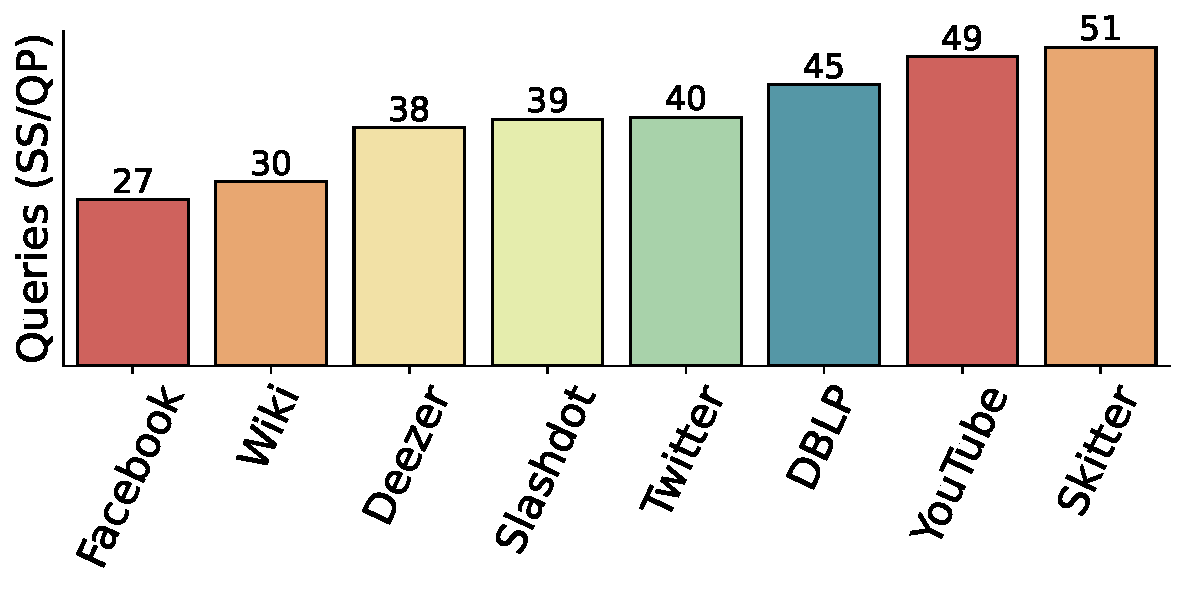
\includegraphics[width=0.7\textwidth]{figures/quickprune/MaxCover_QueriesToPrune.pdf}
  \caption{Oracle calls required by QuickPrune versus Submodular Sparsification (SS) on
    MaxCover across all datasets. QuickPrune requires orders of magnitude fewer oracle
    calls than SS.}
  \label{fig:qp-oracle}
\end{figure}

\subsection{Results on Knapsack Constraints}

For general knapsack constraints, where the cost of each node is set proportional to its
degree following~\citep{yaroslavtsev2020bring}, we compare QuickPrune against Top-$k$
(which selects elements with the highest degree-to-cost ratios) and GNNPruner.
Figure~\ref{fig:qp-knapsack-violin} shows the distribution of the combined metric $C$
across all eight SNAP datasets for each problem. QuickPrune exhibits consistently high
performance with low variance across all three problems, achieving a mean $C$ above 0.9
for both MaxCover and MaxCut. In contrast, Top-$k$ and GNNPruner show high variance,
performing well on some instances but poorly on others. For Influence Maximization, Top-$k$ is competitive with QuickPrune on average, but its
poor performance on MaxCover and MaxCut demonstrates limited robustness across problems. GNNPruner suffers from
the most inconsistent behavior, with $C$ values ranging from near-zero to near-perfect
depending on the dataset.

\begin{figure}[t]
  \centering
  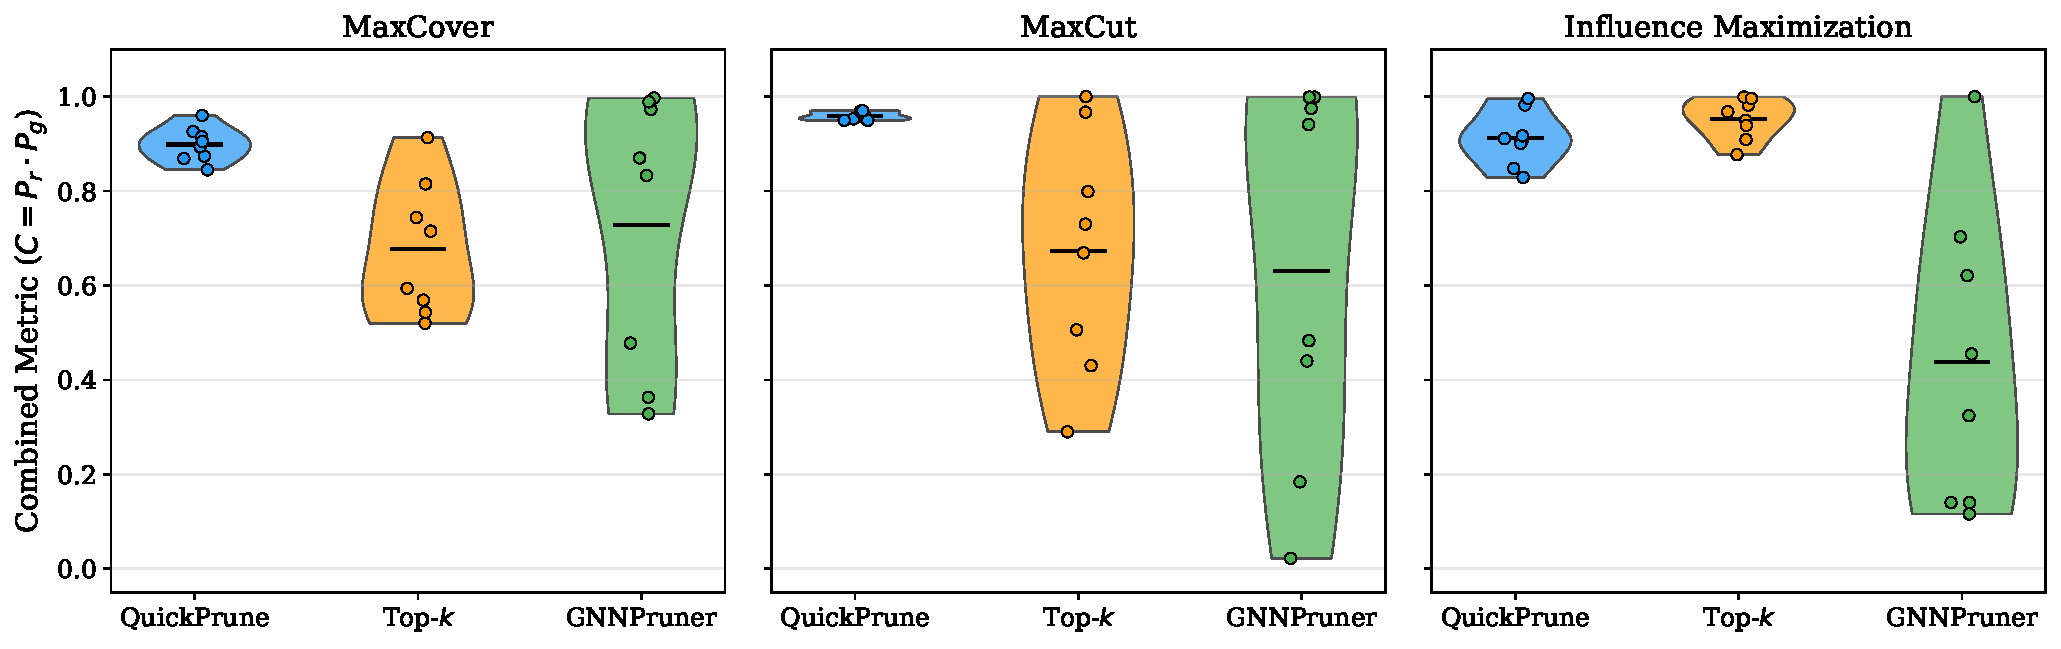
\includegraphics[width=\textwidth]{figures/quickprune/knapsack_violin.pdf}
  \caption{Distribution of the combined metric $C = P_r \cdot P_g$ under knapsack
    constraints across eight SNAP datasets. Each point represents one dataset. QuickPrune
    maintains consistently high performance with low variance, while Top-$k$ and GNNPruner
    exhibit high variance across datasets and problems.}
  \label{fig:qp-knapsack-violin}
\end{figure}

\subsection{Multi-Budget versus Single-Budget Comparison}

We compare QuickPrune (multi-budget) with QuickPrune-Single (which prunes for the
maximum budget only) for a range of budgets from $10$ to $100$. For size constraints, no
significant improvement is observed for QuickPrune over QuickPrune-Single, likely due to
the efficacy of the standard greedy algorithm for size constraints, where a greedy
solution of smaller size is automatically contained in greedy solutions of larger sizes.
However, for general knapsack constraints, QuickPrune typically improves by 3-10\% over
QuickPrune-Single for Influence Maximization, while increasing the size of the reduced
ground set by less than 1\%. Similar improvements are observed on some datasets for
MaxCover, while for MaxCut the two variants perform similarly.
Figure~\ref{fig:qp-multiBudget} shows the multi-budget comparison for Influence
Maximization under knapsack constraints across four datasets.

\begin{figure}[t]
  \centering
  \begin{subfigure}[b]{0.24\textwidth}
    \centering
    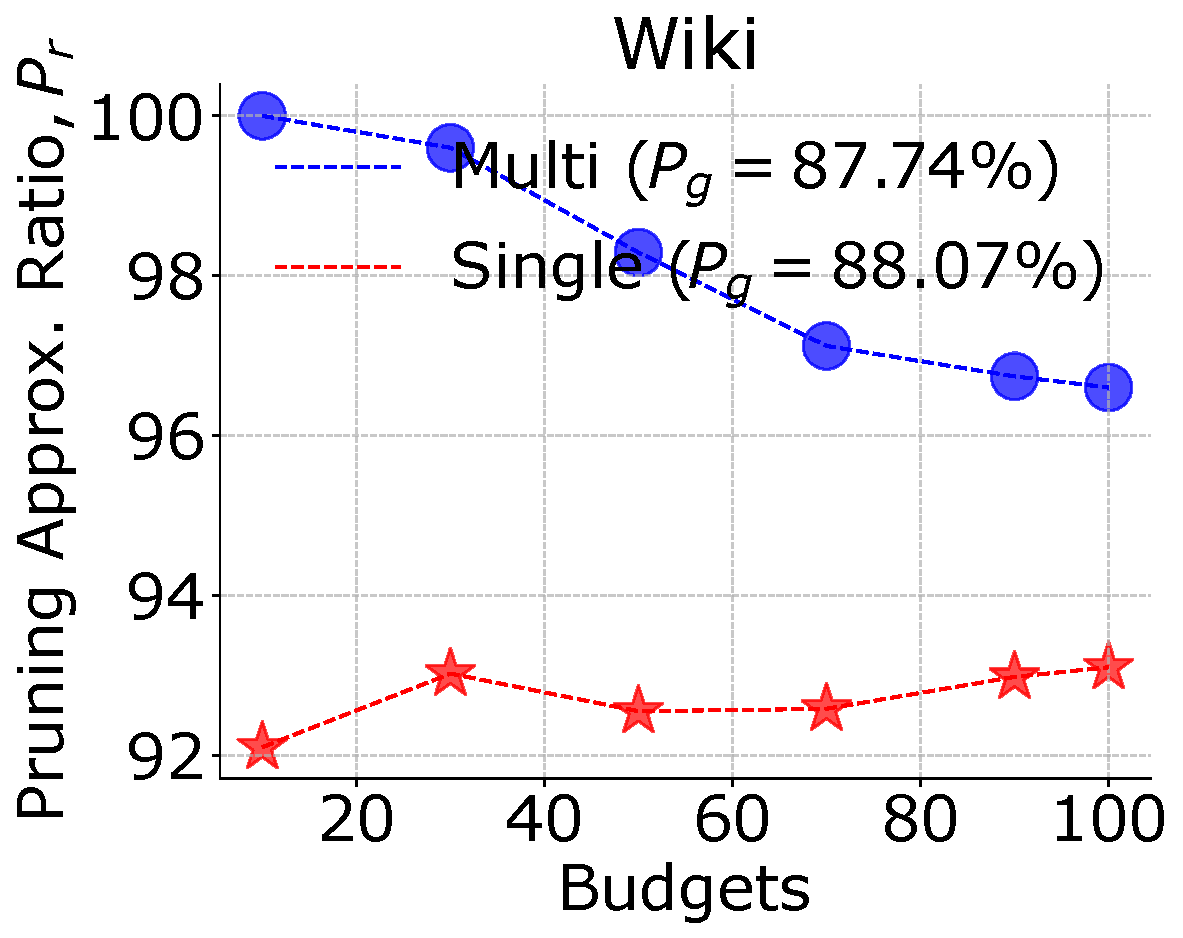
\includegraphics[width=\textwidth]{figures/quickprune/IM_Wiki.pdf}
    \caption{Wiki}
    \label{fig:qp-im-wiki}
  \end{subfigure}
  \hfill
  \begin{subfigure}[b]{0.24\textwidth}
    \centering
    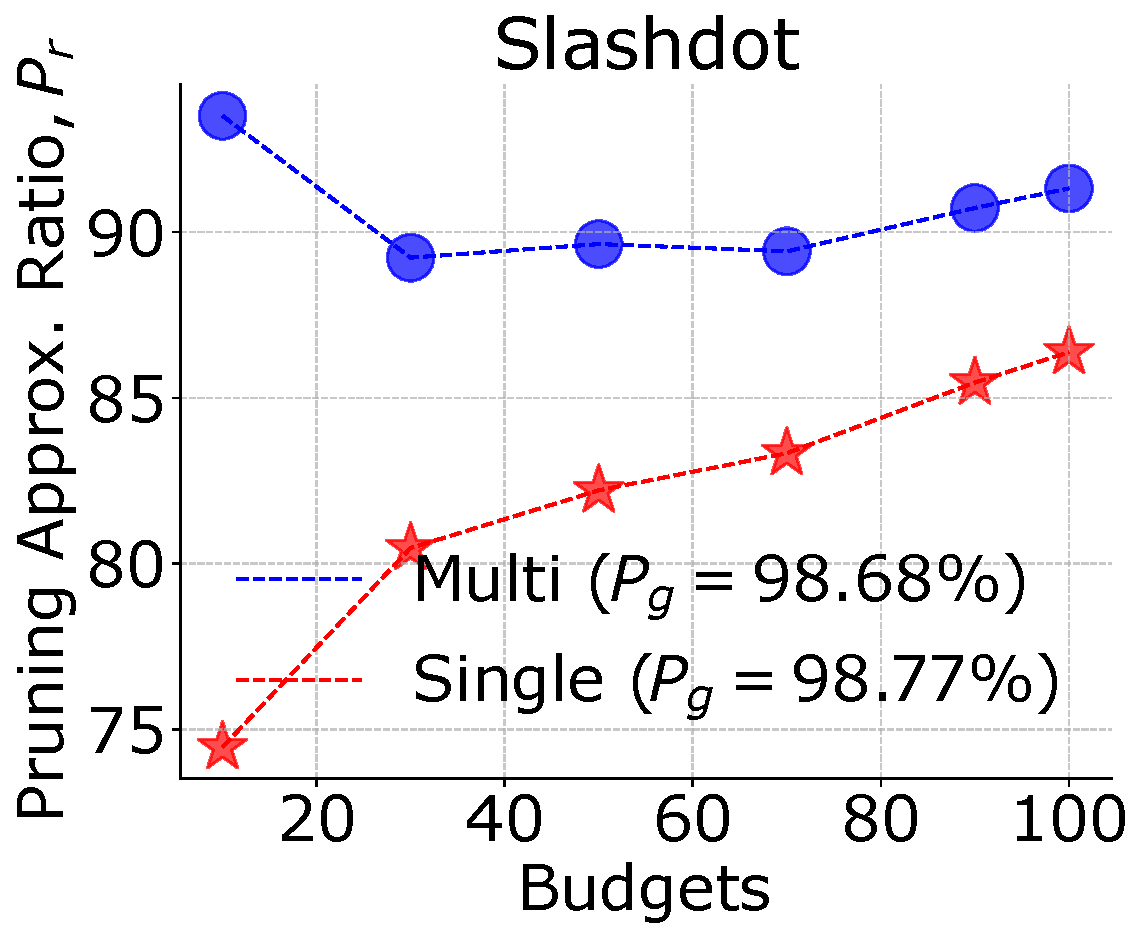
\includegraphics[width=\textwidth]{figures/quickprune/IM_Slashdot.pdf}
    \caption{Slashdot}
    \label{fig:qp-im-slashdot}
  \end{subfigure}
  \hfill
  \begin{subfigure}[b]{0.24\textwidth}
    \centering
    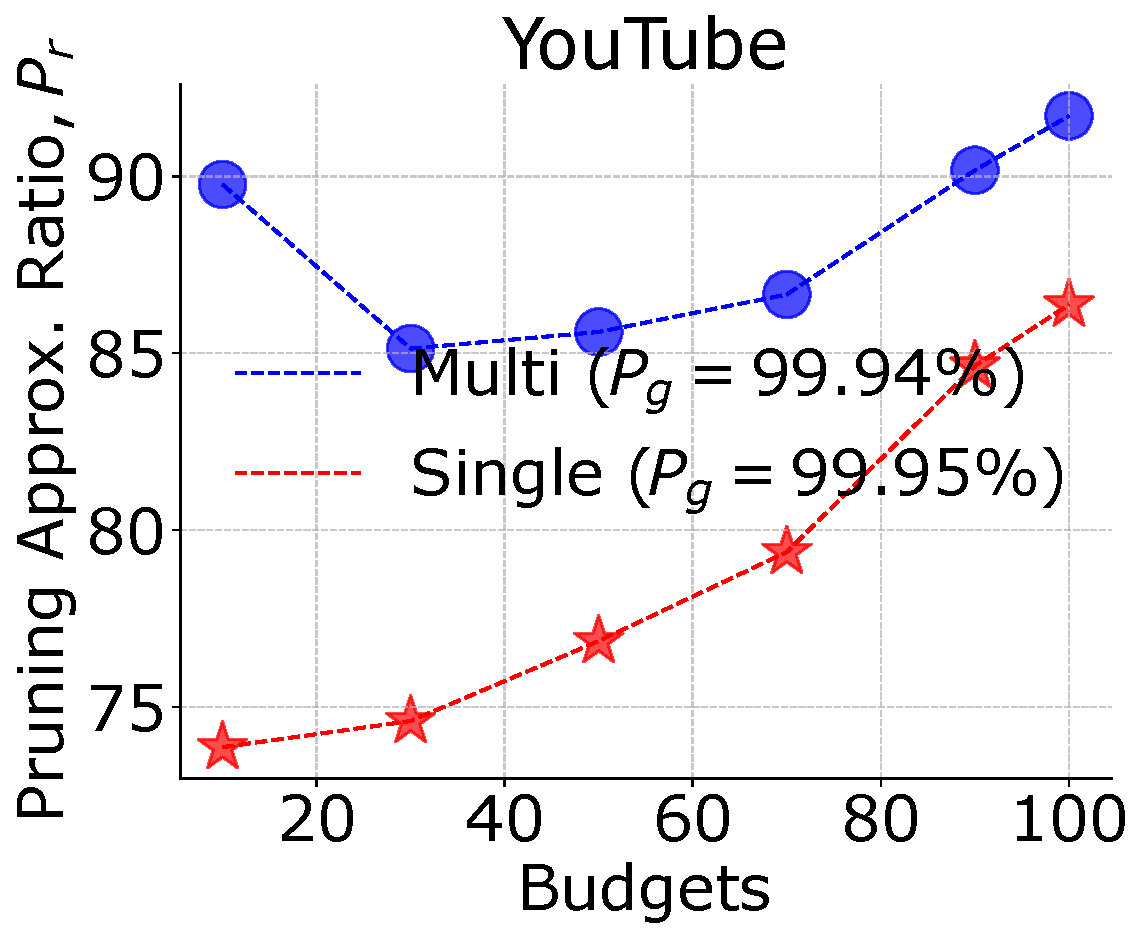
\includegraphics[width=\textwidth]{figures/quickprune/IM_YouTube.pdf}
    \caption{YouTube}
    \label{fig:qp-im-youtube}
  \end{subfigure}
  \hfill
  \begin{subfigure}[b]{0.24\textwidth}
    \centering
    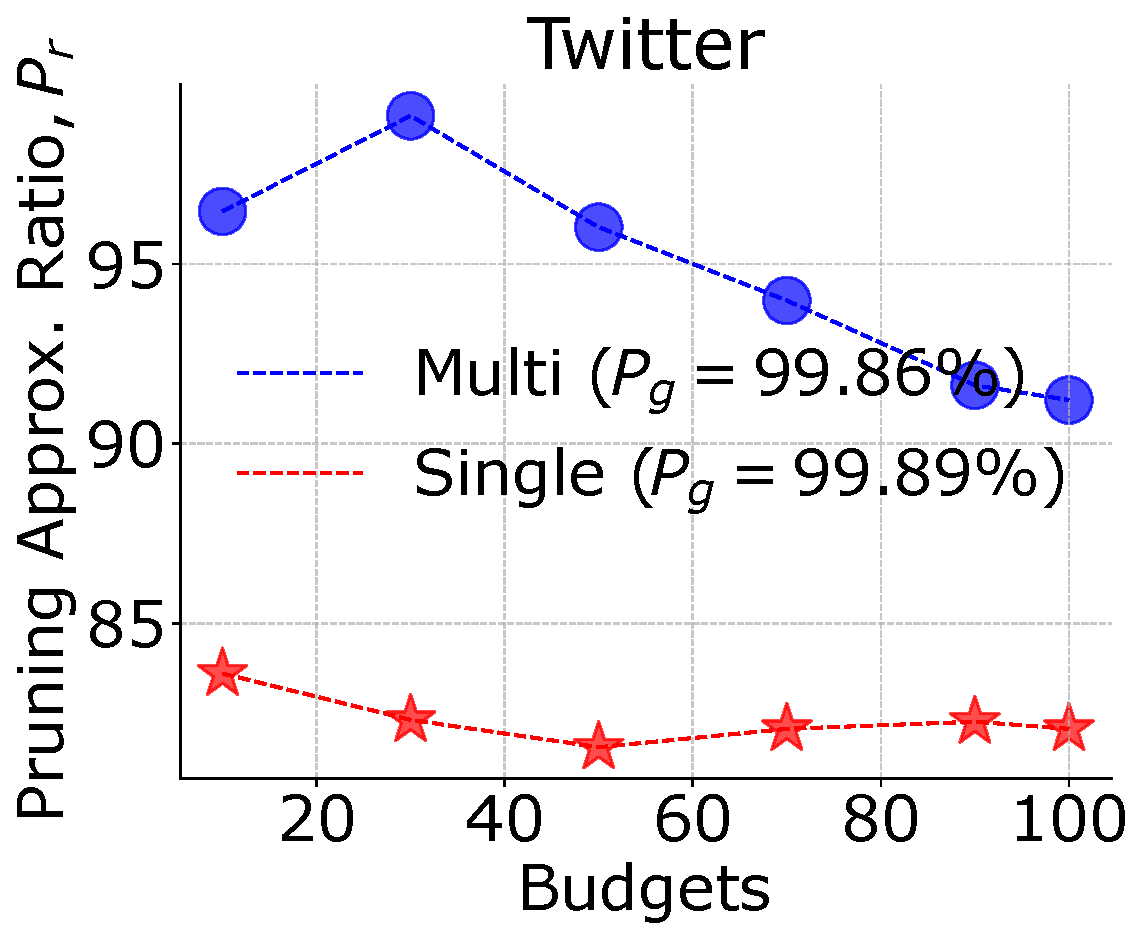
\includegraphics[width=\textwidth]{figures/quickprune/IM_Twitter.pdf}
    \caption{Twitter}
    \label{fig:qp-im-twitter}
  \end{subfigure}
  \caption{Multi-budget vs.\ single-budget comparison for Influence Maximization under
    knapsack constraints. QuickPrune (multi-budget) consistently improves over
    QuickPrune-Single across a range of budgets from 10 to 100.}
  \label{fig:qp-multiBudget}
\end{figure}

\section{Discussion}

\textbf{Theory-empirical gap.}
For natural parameter choices ($\gamma = 1$, $\delta = 1$, $\epsilon = 0.01$), Theorem~2
gives a value retention constant of $(1-0.01)/24 \approx 0.041$, guaranteeing retention of
at least roughly $4\%$ of the optimal value. Empirically, however, QuickPrune achieves
$P_r \approx 0.96$-$1.00$ across all benchmarks, a gap of more than $20\times$.
This is an artifact of worst-case analysis: the bound must hold for all
$\gamma$-weakly submodular functions and all element orderings, so each step of the proof
introduces slack that real instances do not exhibit. 
